% Chapter 5

\chapter{Document Clustering} % Main chapter title

\label{clustering} % For referencing the chapter elsewhere, use \ref{Chapter4} 

\lhead{Chapter 5. \emph{Document Clustering}} % This is for the header on each page - perhaps a shortened title

%----------------------------------------------------------------------------------------
In this chapter we discuess the choosed clustering algorithms and implementation details, An introduction to document clustering is provided in section ~\ref{sec:intro}, section \ref{sec:background} introduces the dynamic modeling and distance relatedness concepts which are used in the Mitosis algorithm, Mitosis distance relatdness model is introduced in section ~\ref{sec:mitosis_proposed}, algorithms steps are explained in section ~\ref{sec:phases}, where implementation details are given in section ~\ref{sec:implementation}

\section{Introduction} \label{sec:intro}
Document clustering has been investigated for use in a number of different areas of text
mining and information retrieval. Initially, document clustering was investigated for improving
the precision or recall in information retrieval systems and as an efficient way of
finding the nearest neighbors of a document. More recently, clustering has been
proposed for use in browsing a collection of documents or in organizing the results
returned by a search engine in response to a user's query. Document clustering has
also been used to automatically generate hierarchical clusters of documents. (The
automatic generation of a taxonomy of Web documents like that provided by Yahoo! \citep{clustering_15}

In this work we used clustring to group similar articles together for to ease user browsing and to determine the user neighborhood to enhance the performance of the system as we don't need to use all users' profiles in the system in the recommendation algorithm to determine the recommendations to a specified user, but instead we only investigate the profiles of the user's neighborhood which are other users who are in the same cluster.

Partitioning algorithms as K-Means \citep{clustering_1}, itsvariants \citep{clustering_2} \citep{clustering_3}, K-Medoids \citep{clustering_4}, PAM \citep{clustering_5} (Partitioning AroundMedoids),BIRCH \citep{clustering_6} and
CLARANS \citep{clustering_7}, tend to use a center-based clustering objective,re-sulting in clusters of known geometrical shape,e.g. asphereoran ellipse. Grid based clustering algorithms include STING \citep{clustering_8}, CliQue \citep{clustering_9},WaveCluster \citep{clustering_10}, andDenClue \citep{clustering_11}.
However,density-based
algorithms asDBScan \citep{clustering_12}, DenClue \citep{clustering_11}, andSNN(SharedNear-
est Neighbors) \citep{clustering_13} have introduced new clustering criteria that do not restrict the shape of clusters, and thus are able to obtain what is called \textit{arbitrary} shaped clusters.
Yet,they depend on using a static model for clustering, which deteriorates when arbitrary densities are present in data. Chameleon  \citep{clustering_14}, on the
other hand, uses a dynamic model to be able to merge clusters of related densities together. Yet, Chameleon suffers some drawbacks.

\section{DBSCAN}
DBSCAN stands for \textbf{D}ensity-\textbf{B}ased \textbf{S}patial \textbf{C}lustering of \textbf{A}pplications with \textbf{N}oise, it is a denisty based clustering algorithm which uses the concepts of density reachability and density connectivity\citep{literature_1} as showed in chapter ~\ref{literature}, DBSCAN works as followos
\subsection{The algorithm:}
\citep{literature_2}  The key idea of the DBSCAN algorithm is that, for each point of a cluster, the neighbourhood 
of a given radius has to contain at least a minimum number of points, that is, the density in 
the neighbourhood has to exceed some predefined threshold. This algorithm needs three 
input parameters:
\begin{itemize}  
\item{$k$, the neighbour list size} 
\item{$Eps$, the radius that delimitate the neighbourhood area of a point ($Eps_neighbourhood$)}
\item{MinPts, the minimum number of points that must exist in the Eps-neighbourhood.}
\end{itemize} 

In our work $k$ is obtained by \textit{first} constructing a similarity matrix between all pairs of documents using one of the techniques explained in chapter ~\ref{sim}, the similarity matrix is stored in a database where for each document its id, location and source are stored too. Adter that for each document if the number of neighbours that are not more than $Eps_neighbourhood$ apart is greater than $MinPts$ they are considered as one cluster.

\section{Mitosis}
For the shortcomings of other clustering algorithms mentioned above we applied the model proposed in \textbf{Mitosis} \citep{Mitosis_1} which introduces a dynamic model based on distance relatedness concepts to overcome drawbacks of related algorithms. Mitosis discovers clusters of arbitrary shapes and densities. It uses distance relatedness between patterns (in this case documents)as a measure to identify clusters of different densities.
Mitosis overcomes the traditional clustering algorithms in the following points.
\begin{itemize}
\item{Combining both local and global novel distance-consistency measures in a dynamic model to cluster the data.}
\item{Introducing a greedy clustering approach to keep up with the linear time performance of simple algorithms.}
\item{The ability to identify outliers in the presence of clusters of different densities in the same dataset.}
\item{The use of a parameter selection procedure to guide the clustering algorithm.}
\item{Suitability for high dimensional data, where the discovery of arbitrary shape and density clusters reveals other relations not revealed by traditional clustering algorithms.}
\end{itemize}
The following subsection will introduce the background needed to explain the algorithm.
\subsection{Dynamic modeling and distance relatedness concepts}\label{sec:background}

The significance of a dynamic model of clustering is first explained ~\ref{subsec:dynamic_static}, and the theoretical background of distance relatedness is then discussed ~\ref{subsec:dist_density}.

\subsubsection{Dynamic vs. static models}\label{subsec:dynamic_static} 
A static model refers to using user-defined parameters for defining density thresholds without referring to the characteristics of the underlying data.DBScan, DenClue, WaveClusterandSNN, are examples of algorithms that use a static model and are unable to find clusters of arbitrary densities.For example, DBScan uses two parameters \textit{Eps} and \textit{Minpts}, where \textit{Eps} specifies a threshold on range distance,
and Minpts specifies the minimum number of neighbors.
Apattern with a number of neighbors more than Minpts at adistance less than Eps, is considered a corepoint(\textit{pattern}) and is used to track clusters. Chameleon,on the other hand introduced a dynamic modelfor
clustering based on the following:
\begin{itemize}
\item The use of k-nearest neighbors(\textit{k-NN}).
\item Merging of clusters based on relative closeness and relative interconnectivity measures, weighed by user defined parameters.
\end{itemize}


\subsubsection{Distance-based density}\label{subsec:dist_density} 
Clusters can be visually detected by recognizing relatively higher density regions in data separated by regions of relatively lower densities. It is observed that the behavior of neighborhood distances determines the degree of a cluster's density; smaller distances reflect higher densities, and viceversa. The average distances between patterns(the Minimum
Spanning Tree(\textit{MST}) distances) differentiate the densities of clusters in Fig. ~\ref{fig:mitosis_1}. Several other points important to build an efficient model are as follows:
\begin{itemize}
\item Arbitrary shaped clusters can be detected by tracking connectivity between patterns' neighborhoods.
\item The distances between a pattern and its neighbors determine the density of its cluster.
\item Patterns of the same cluster, should have consistent neighborhood distances to preserve a consistent density thoughout the cluster.
\end{itemize}
\textbf{Distance relatedness measures:} Local and global measures for distance relatedness have been separately considered for clustering. Local relatedness refers to relatedness of distances in two neighboring patterns' neighborhoods, while global relatedness refers to relatedness of distances in a group of patterns' neighborhoods to those in a neighboring group's neighborhoods. Thus global relatedness considers relating the neighborhoods of two patterns that may not be in each other's neighborhoods, but can be reached from one another through a group of neighbor patterns. Global distance relatedness does not guarantee local distance relatedness. Yet considering both local and global relatedness aims at increasing the distance consistency of each cluster, and avoiding the effect of outliers which may merge two clusters together.

\begin{figure}[htbp]
	\centering
		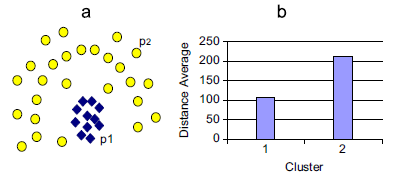
\includegraphics{./Figures/Mitosis_1.png}
		\rule{35em}{0.5pt}
	\caption[Distances between patterns reflect the density structure.]{Distances between patterns reflect the density structure.}
	\label{fig:mitosis_1}
\end{figure}

\subsection{Mitosis Proposed distance relatedness dynamic model}\label{sec:mitosis_proposed}
The dynamic model proposed in \textit{Mitosis} aims at maintaining the consistency of distances between patterns in each cluster.It defines a
distance-relatedness clustering criterion based on the following:
\begin{itemize}
\item A dynamic range neighborhood that depends on the density context of the pattern.
\item Measures that reflect the distance structure of the data.
\end{itemize}

Mitosis distance relatedness model combines both local and global distance relatedness. 
It attempts to cluster the data starting from local measures and extending that to global ones in the course of the algorithm. 
Let the symbols $x$, $y$, $p$, and $q$ denote a pattern, $d(x,y)$ denotes the distance between patterns $x$ and $y$, $a$ denotes the association between two patterns $x$ and $y$, which is the tuple $(x,y,d(x,y))$, $A$ denotes a set of associations, $f$ and $k$ denote user parameters, and $\mu$ denotes the average value of distances.

\textbf{Local distance relatedness}: Any cluster is initially formed from singleton patterns that are related with respect to their neighborhood
average distance measure, and have an in-between distance related to this measure as well. This local merging criterion is a modification of Zahn'sinconsistencymodel.
The rules proposed here are as follows, considering that an average local distance measure is the average of distances in a neighborhood of a pattern as given later
\begin{itemize}
\item The distance between two patterns is related to each of the patterns' average local distance measure, by a factor k.
\item The two patterns' average local distance measures are related by factor k.
\end{itemize}

Figure ~\ref{fig:mitosis_2} illustrates the importance of the mutual consistency between the three entities associated with the local relatedness
criterion; two patterns and a nin-between distance. It shows two examples, the first example ($p_1, p_2, d_1$) has two patterns with distance $d_1$related to each patterns' neighborhood distances, yet the two neighborhood distance averages are not related. The second case ($p_3, p_4, d_2$)gives an example of two related neighborhood distance averages, but an unrelated in-between distance $d_2$. The two patterns do not merge in any of these cases, justifying the above proposed local criterion that imposes the mutual consistency between the two neighborhoods and the in between distance. 
The same rationale is used when merging two clusters, but this time considering the clusters' global characteristics.

\begin{figure}[htbp]
	\centering
		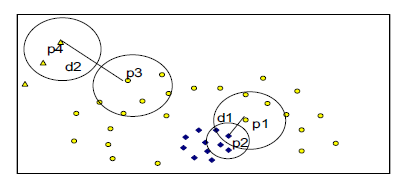
\includegraphics{./Figures/Mitosis_2.png}
		\rule{35em}{0.5pt}
	\caption[Effect of distance inconsistency on merging of patterns]{Effect of distance inconsistency on merging of patterns}
	\label{fig:mitosis_2}
\end{figure}


\textbf{Global distance relatedness}: The property of distance consistency
extends from local relations between neighborhood patterns to global relations between neighboring clusters. The global distance relatedness model follows the same rules of the local relatedness, but with replacing patterns with clusters, a pattern's local average distance with a cluster's average distance, and the distance between two singleton patterns with the distance between the two patterns in the two neighboring clusters. A cluster's average distance(only distances approved to be consistent to the cluster)is used to reflect the distance behavior inside the cluster.

\subsubsection{Distance consistency definitions}
The rules governing consistency of one distance to another cluster's/pattern's average distance, or two clusters'/patterns' average
distance to each other are as follows. given an input parameter $k > 1$:
\begin{itemize}
\item A distance $d(x,y)$ is \textit{k-consistent} to an average $\mu$ of distances if
$d(x, y)<k. \mu$
\item Two distance averages $\mu_1$ and $\mu_2$ are \textit{k-consistent} to each other if $\mu_1 < k.\mu_2 \wedge \mu_2 <k.\mu_1$ or equivalently min$(\mu_1, \mu_2)< k.max(\mu_1, \mu_2)$
\item A distance $d(x,y)$ is \textit{k-consistent} to two averages if $d(x, y)< k.\mu_1 \wedge d(x, y)< k.\mu_2$  i.e. $d(x, y)< k.min(\mu_1, \mu_2)$
\end{itemize}
According to the above definitions the merge criteria are proposed.

\subsubsection{Algorithms phases}\label{sec:phases}

The algorithm takes as an input the dataset $P$, and 2 main parameters $f$ and $k$. The main steps are as follows:
\begin{itemize}

\item {Get associations:
\begin{itemize}
	\item For each pattern get its dynamic range nearest neighbors using parameter $f$, and calculate local average distance.
	\item Order the associations—ascendingly on distances-between patterns inalist L.
\end{itemize}
}


\item {Merge patterns in to clusters: For each association in L (visited in order), if the merging criterion is satisfied—according to k-, merge
associated patterns/clusters, and update the clusters'measures.}
\item {Refine clusters:
\begin{itemize}
\item For each cluster, add any internal association consistent to the cluster'saverage.
\item For each cluster, calculate the Harmonic average of distances, and remove associations not consistent to this measure.
\end{itemize}
}
\end{itemize}


\subsection{Implementation Details}\label{sec:implementation}
The class diagram of the implementation of Mitosis is illustrated in figure ~\ref{fig:mitosis_6} where class \textit{Pattern} is an abstract class represents the object to be clustered, in our work the class \textit{Document} implements it, this class sotores the representation of the document which is an N-dimentional feature vector each pattern has a reference to its cluster.
The \textit{Asscaition} class contains the relations between the pattern \textit{p} and all other patterns within its dynamic range. Each \textit{Cluster} object contains a list of all patterns and associations consisting it, the \textit{Cluster} object contains the mean value of distances of associations in the cluster $\mu$, and keep updating it while more associations is added to it.

\begin{figure}[htbp]
	\centering
		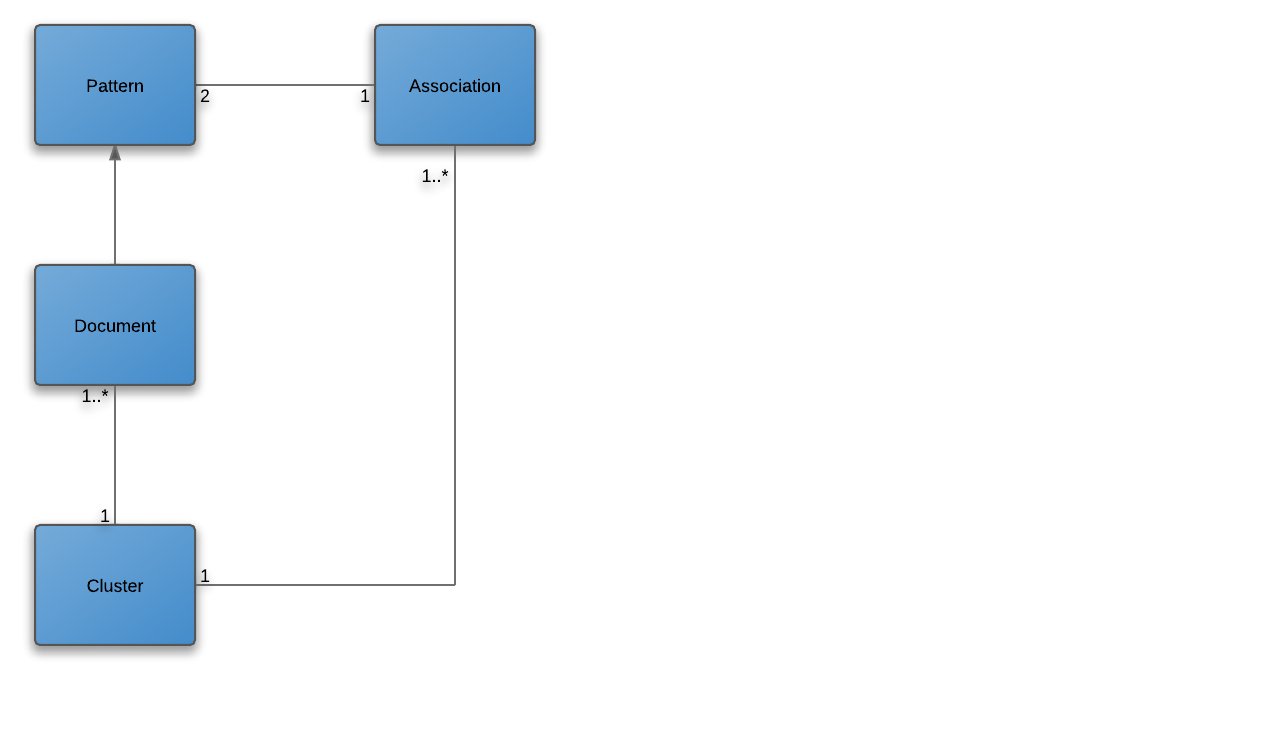
\includegraphics{./Figures/Mitosis_6.png}
		\rule{25em}{0.3pt}
	\caption[Mitosis class Diagram]{Mitosis class Diagram}
	\label{fig:mitosis_6}
\end{figure}

\subsubsection{Loading associations} 
Mitosis requires loading the associations of each pattern which have distance less than $f.min{dist}$ where $f$ is mitosis factor and $min_{dist}$ is the minimum distance betweeen the pattern and all its neighbours.

Given a databse that stores all the distances between all pairs of patterns, loading associations that are in dynamic range for a given patterns $p$ is performed on two steps, first the database is queried to obtain the the nearst pattern to $p$ which is at distance $min{dist}$, then the pattern's threshold is calculated as $threshold_{dist} = f \dot dist_{min}$ the database is queried again to obtain all the association with distance less than or equal to $threshold{dist}$.

The clustering algorithm is first applied on two different sets of 2D points (the data set could be found at \citep{Mitosis_2}) for verifying the correctness of the implementation, the results are illustrated in figures ~\ref{fig:mitosis_7} and ~\ref{fig:mitosis_8}.
\begin{figure}[htbp]
	\centering
		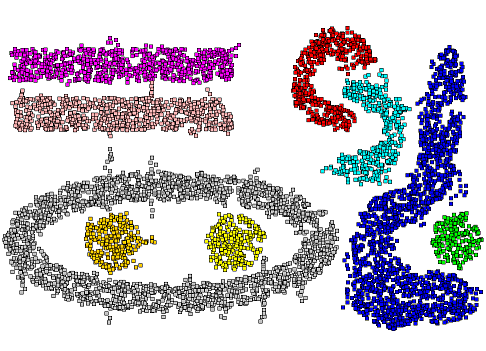
\includegraphics{./Figures/Mitosis_7.png}
		\rule{25em}{0.3pt}
	\caption[Mitosis result on 2D points]{Mitosis result on 2D points}
	\label{fig:mitosis_7}
\end{figure}

\begin{figure}[htbp]
	\centering
		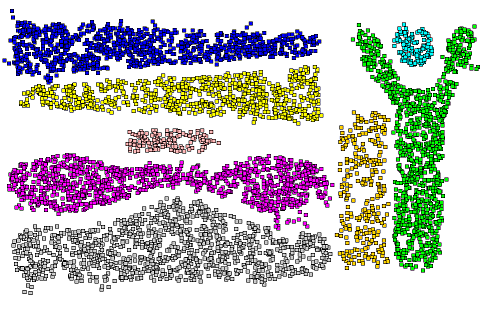
\includegraphics{./Figures/Mitosis_8.png}
		\rule{25em}{0.3pt}
	\caption[Mitosis result on 2D points]{Mitosis result on 2D points}
	\label{fig:mitosis_8}
\end{figure}

Merging phase is a transitive operation, so equivalence classes must be implemented efficiently to avoid any perofrmance bottleneck.
This can be achieved by using \textit{Disjoint sets data structures}
\subsubsection{Disjoint set}

A disjoint-set is a collection $C={S_1, S_2,..., S_k}$ of distinct dynamic sets.
Each set is identified by a member of the set, called representative.
Disjoint set operations:
\begin{itemize}
\item MAKE-SET(x): create a new set with only x. assume x is not already in some other set.
\item UNION(x,y): combine the two sets containing x and y into one new set. A new representative is selected.
\item FIND-SET(x): return the representative of the set containing x.
\end{itemize}
Obviously the \textit{MAKE-SET(x)} operation can be used at the beginning of the algorithm as each pattern will be in a cluster, and the \textit{UNION(x,y)} will be used to marge to clusters.
Next sub-sections will illustrate different implementations
\paragraph{Linked-List Implementation}
Each set as a linked-list, with head and tail, and each node contains value, next node pointer and back-to-representative pointer.
Figure ~\ref{fig:mitosis_3} ~\ref{fig:mitosis_4} shows the operations of the disgoint set.
\begin{itemize}
\item MAKE-SET costs \BigO{1}: just create a single element list.
\item FIND-SET costs \BigO{1}: just return back-to-representative pointer.
\item {UNION(x,y) 
\begin{itemize}
\item {A simple implementation: just appends x to the end of y, updates all back-to-representative pointers in x to the head of y.
Each UNION takes time linear in the x’s length}
\item {Instead appending x to y, appending the shorter list to the longer list.
Associated a length with each list, which indicates how many elements in the list.
}
\end{itemize}
}
\end{itemize}

\begin{figure}[ht]
\begin{minipage}[b]{0.5\linewidth}
\centering
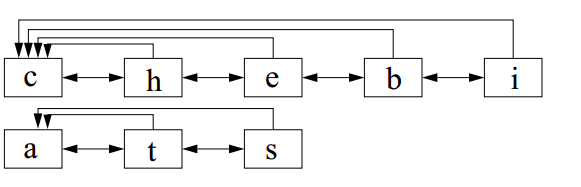
\includegraphics[width=\textwidth]{./Figures/Mitosis_3.png}
\caption{Two sets}
\label{fig:mitosis_3}
\end{minipage}
\hspace{0.5cm}
\begin{minipage}[b]{0.5\linewidth}
\centering
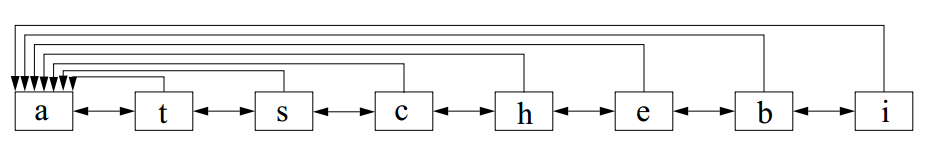
\includegraphics[width=\textwidth]{./Figures/Mitosis_4.png}
\caption{Union of two sets}
\label{fig:mitosis_4}
\end{minipage}
\end{figure}

\paragraph{Disjoint-set Implementation: Forests}
Rooted trees, each tree is a set, root is the representative. Each node points to its parent. Root points to itself.

Three operations
\begin{itemize}
\item MAKE-SET(x): create a tree containing x.  \BigO{1}
\item FIND-SET(x): follow the chain of parent pointers until to the root. \BigO{height of x’s tree}
\item UNION(x,y): let the root of one tree point to the root of the other.  \BigO{1}
\end{itemize}

\textbf{Union by Rank and  Path Compression}
\textit{Union by Rank}: Each node is associated with a rank, which is the upper bound on the height of the node (i.e., the height of subtree rooted at the node), then when UNION, let the root with smaller rank point to the root with larger rank. 
\textit{Path Compression}: used in FIND-SET(x) operation, make each node in the path from x to the root  directly point to the root. Thus reduce the tree height.

\begin{figure}[htbp]
	\centering
		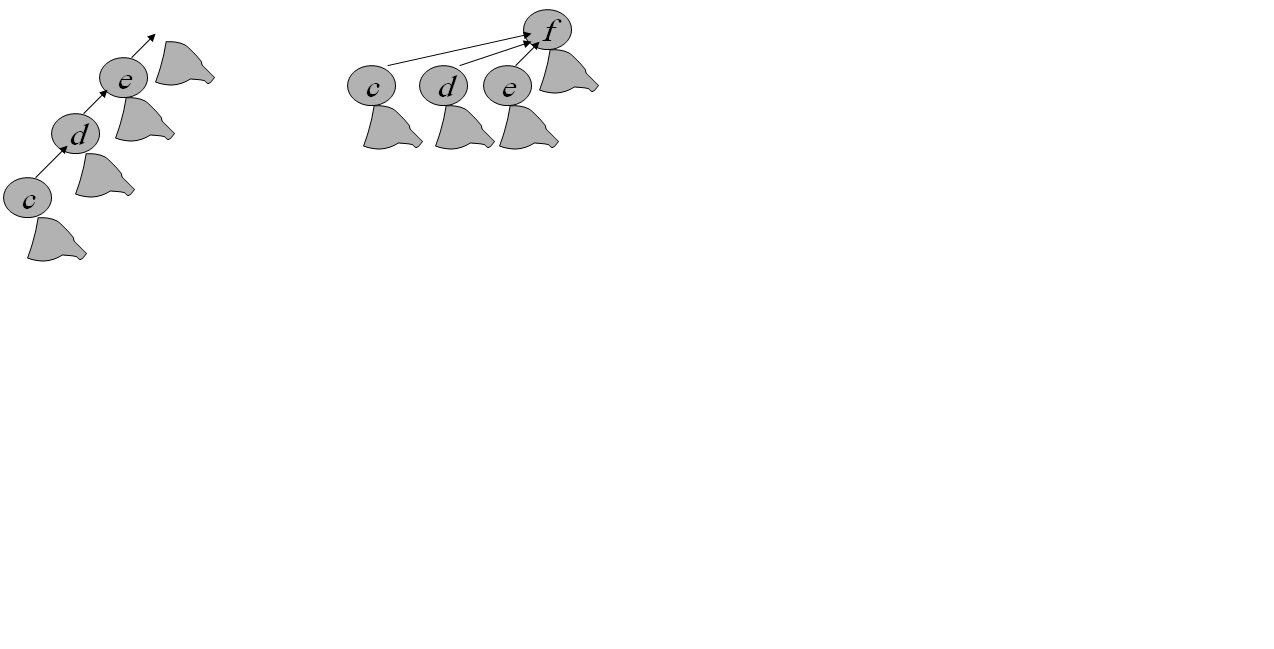
\includegraphics{./Figures/Mitosis_5.png}
		\rule{25em}{0.3pt}
	\caption[Path compression]{Path compression}
	\label{fig:mitosis_5}
\end{figure}
%----------------------------------------------------------------------------------------

